\documentclass{report}
\usepackage[utf8]{inputenc}
\usepackage{amsmath}
\usepackage{qtree}
\usepackage{tikz}
\title{This is the document's title}
\author{J.~Doe}
\date{Today's Date}

\begin{document}
\Tree[.\text{Frog is at lily pad 2} [
        [
                .\text{Lose (Go to lily pad 1)}
                \text{Eventually Win ($P(1)$)}
                \text{Eventually Lose ($P(1)'$)}
            ]
            [
                .\text{Win (Go to lily pad 3)}
                \text{Eventually Win ($P(3)$)}
                \text{Eventually Lose ($P(3)'$)}
            ]
    ]]




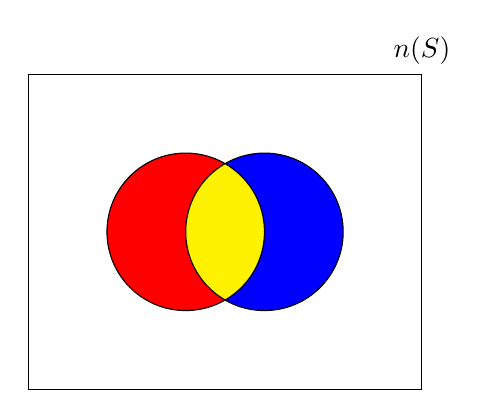
\begin{tikzpicture} % [scale=2]
    \filldraw[fill=white] (-2,-2) rectangle (3,2);

    % First circle (A)
    \fill[red] (0,0) circle (1);

    % Second circle (B)
    \fill[blue] (1,0) circle (1);

    % Intersection of the circles
    \begin{scope}
        \clip (0,0) circle (1);
        \fill[yellow] (1,0) circle (1);
    \end{scope}

    % outline of circles & labels
    \draw (0,0) circle (1);
    \draw (1,0) circle (1);
    % \node [above] at (0,1) {$\text{Bs Touch}$};
    % \node [above] at (1,1) {$\text{Is Touch}$};

    % Outline of the rectangle with label
    \draw (-2,-2) rectangle (3,2) node [above] {$n(S)$};
\end{tikzpicture}

\end{document}